
\documentclass[onehalf,11pt]{beavtex}
\title{The Meaning of Life}
\author{John Smith}
\degree{Doctor of Philosophy}
\doctype{Dissertation}
\department{Electrical Engineering and Computer Science}
\depttype{School}
\depthead{Director}
\major{Computer Science}
\advisor{Joan Smythe}
\submitdate{September 23, 2011}
\commencementyear{2012}
\abstract{This is an abstract statement.}
\acknowledgements{I would like to acknowledge the Starting State and the Transition Function.}

\usepackage{algorithm}
\usepackage{algorithmic}
\usepackage{graphicx}
\usepackage{grffile}
\usepackage{amsmath}
\usepackage{amssymb}
\usepackage{times}
\usepackage{epsfig}
\usepackage{breqn}
\usepackage{url}
\usepackage[lined,boxed,commentsnumbered,algo2e]{algorithm2e}

\begin{document}
\maketitle

\mainmatter

\chapter{Introduction}
I have done some excellent research \cite{matrix}.
\section{Introduction to the Introduction}
\begin{figure}[!ht]
\centering
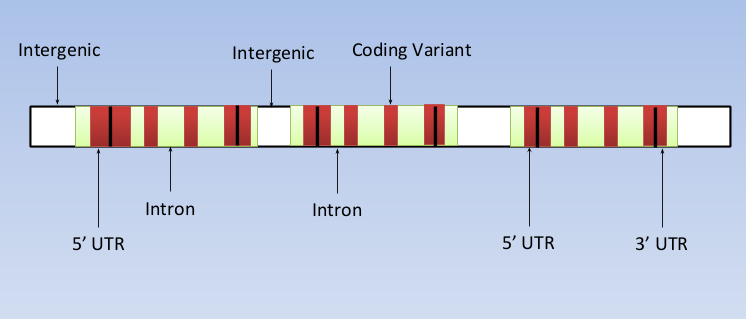
\includegraphics[scale=0.6]{./pic/type.png}
\caption{}
\end{figure}


\chapter{Methods}

\section{Input}

\subsection{Genome data}
A faidx-indexed reference file in the FASTA format. It consists of the whole nucleotide sequences of each chromosome. We will use this file to get the amino acid codon of a given variant.
Example:

\begin{figure}[!ht]
\centering
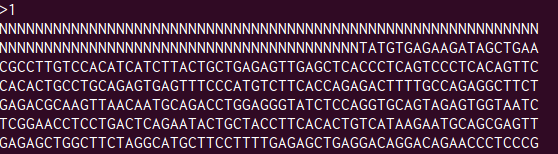
\includegraphics[scale=0.8]{./pic/genome.png}
\caption{Genome data example}
\end{figure}

\subsection{Gene structure data}
A GTF formatted file that is used to hold information about gene structure. It is a tab-delimited text format based on the general feature format (GFF), but contains some additional conventions specific to gene information. The key information is the start and stop positions of genes and Coding sequences. We will use this file to determine the functional area of a given variant. Example:

\begin{figure}[!ht]
\centering
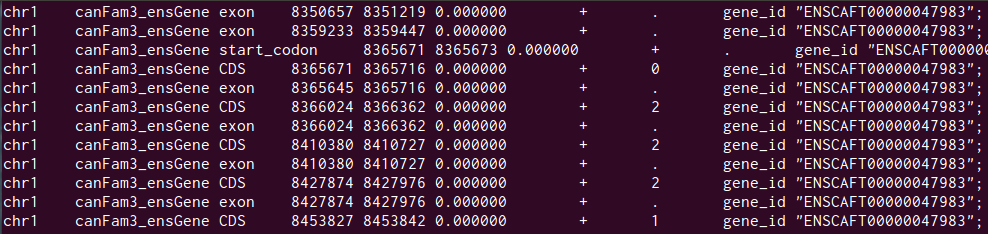
\includegraphics[scale=0.6]{./pic/gtf.png}
\caption{GTF file example}
\end{figure}




\subsection{Variant data}
A variant file in VCF format.  This is the file to be annotated. The key information includes chromosome, position reference base and alternate variant alleles of the variant. We will annotate the variants in the INFO field. Example:
\begin{figure}[!ht]
\centering
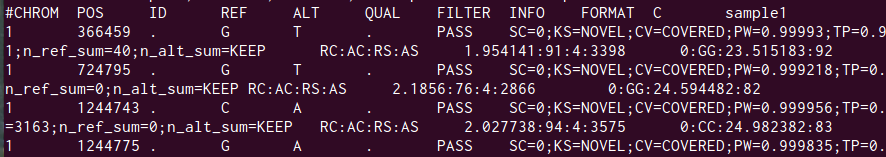
\includegraphics[scale=0.6]{./pic/vcf.png}
\caption{VCF file example}
\end{figure}


\section{Output}
We will annotate the input VCF file in the INFO field and output it as another VCF file. To be specific, a new subfield, named ANN, will be appended to INFO field. The most important information is the effect of variants and the putative impact of the effect. The possible effect and corresponding impact are shown below.

\begin{table}[H]
%\label{tab:features}
\centering
\begin{tabular}{l| l}
\hline
Variant effect & Putative impact \\
\hline
  intergenic\_region & MODIFIER \\
  intron\_variant & MODIFIER \\
  5\_prime\_UTR\_variant & MODIFIER \\
  3\_prime\_UTR\_variant & MODIFIER \\
  non\_coding\_exon\_variant & MODIFIER \\
  synonymous\_variant & LOW \\
  non\_synonymous\_variant & MODERATE \\

\end{tabular}
\end{table}

For non-synonymous variant, we annotate the reference amino acid, alternate amino acid and the position of the amino acid instead of the term.

Besides the effect of variants, the corresponding Ensemble transcript id and common gene name are also annotated. All the annotation formats follow the standard variant annotation in VCF format. Example:
\begin{figure}[!ht]
\centering
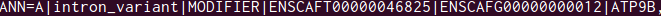
\includegraphics[scale=0.7]{./pic/ann.png}
\caption{VCF file example}
\end{figure}

\section{How it works}
There are 3 files to be kept track of. If we search the whole files for each variants, the total running time complexity is O(m*n*k), where m, n and k is the size of each file. In addition, the size of the files maybe too large to load them all into RAM. For instance, the size of a typical human genome file is about 3.0 GB. To solve the difficulties in this problem, we develop a fast and memory-efficient algorithm to annotate variants.

The whole problem is split into 2 basic subproblem. The first one is to find the functional area of a variant at given chromosome and position. And the second one is to find out the corresponding DNA sequence around the variant and translate it into amino acids, if the variant is inside an exon.

To speed up the annotation, all the 3 files need to be sorted first by chromosome, then by position, in ascending order. Then, the algorithm starts to annotate each variant in the VCF file. When annotating a variant, the algorithm keeps track of the gene area that the variant is in for the next variant to start annotating.

A special problem when annotating is that genes and exons may overlap. So a variant may have multiple distinct annotations. In this case, we need to continue searching until the current gene area is beyond the current variant position. But we still keep track of the first gene area for next annotation.

To save RAM usage, the algorithm only load one chromosome sequence of the DNA data into memory at the same time. This is because no genes overlap on different chromosomes.



\IncMargin{1em}
\begin{algorithm}[h!]
 \label{alg:ANN}
 \SetAlgoLined
 \SetKwData{Left}{left}\SetKwData{This}{this}\SetKwData{Up}{up}
 \SetKwInOut{Input}{input}\SetKwInOut{Output}{output}
 \Input{A GTF file $G$ grouped by gene id. A reference genome file $R$. A VCF file $V$ sorted first by chomosome then by position.}
 \Output{An annotated VCF File}

     \BlankLine
     \For {each variant in V at chromosome chr and position pos}{
		\If{current chromosome $!=$ chr}{
	   		load chr
	  	}
	  	 \BlankLine
	  	\While {$pos$  $>$ the end of current gene}{
	  		 load next gene
	  	}
	  	\BlankLine
	  	
	  	$A$ = $\varnothing$
	  	
	  	\If{ $pos$ $<$ the start of current gene }{
	  		$A$ = $A$ + "intergenic"
	  	}
	  	\BlankLine
	  	
	  	$g$ = current gene\\
	  	\While { $pos$ $>$ the start of $g$ } {
	  		\If{ $g$ has neither start codon nor stop codon}{
	  			$A$ = $A$ + "non coding"
	  		}
	  		\ElseIf{$pos$ not in exon of $g$}{
	  			$A$ = $A$ + "intron"
	  		}
	  		\ElseIf{$pos$ $<$ start codon of $g$}{
	  			$A$ = $A$ + "5' UTR"
	  		}
	  		\ElseIf{$pos$ $>$ stop codon of $g$}{
	  			$A$ = $A$ + "3' UTR"
	  		}
	  		\Else{
	  			get reference amino acid $ra$ and alternative amino acid $aa$\\
	  			\If{ $ra$ == $aa$ }{
	  				$A$ = $A$ + "synonymous"
	  			}
	  			\Else{
	  				$A$ = $A$ + "$ra$ + $pos$ + $aa$"
	  			}
	  		}
	  		$g$ = next gene
	  	}
	  	\BlankLine
	  	Annotate variant with $A$
     }
 \Output{ The annotated VCF file}
 \caption{\textsc{Variant Annotation}}
\end{algorithm}\DecMargin{1em} 

\section{Other issues}
\subsection{how to get amino acid}

\subsection{strand}
%\ref{alg:learning}).

\chapter{Result}

\section{Running time}

\section{Memory cost}

\section{success rate}
\bibliographystyle{plain}
\bibliography{thesis}

\appendix
\chapter{Redundancy}
This appendix is inoperable.

\end{document}
